\renewcommand{\baselinestretch}{1.5}
\chapter{User Guide}
\label{App:UserGuide}

The comparison engine project consists of 3 parts; hardware, device logic, and host software. Using this system involves a number of steps initially setting up each part, and then a simple command line program to run the comparison.

\section{Getting the Code}
All code and resources for this project are available on request from jcr09@ic.ac.uk.

\section{Setting up the Hardware}

The first step required in using the comparison engine is to set up the hardware. This involves connecting the FGPAs together, this is done as detailed in the hardware section of the report (Section 1, Chatpter \ref{chap:design}). This requires connecting each FPGA to the next with ribbon cable as shown in the figures on the next page. Shown on the next page is the setup for the DE0 cluster. A UART must be connected to 1 FPGA, the master device. This is most commmonly done with a UART-USB connector such as the FTDI USB-RS232 cable listed in the bibliography here as reference \cite{FTDI}. Only the TX and RX connectors are needed, the flow control signals can be left unconnected.

 
\begin{figure}[p]
  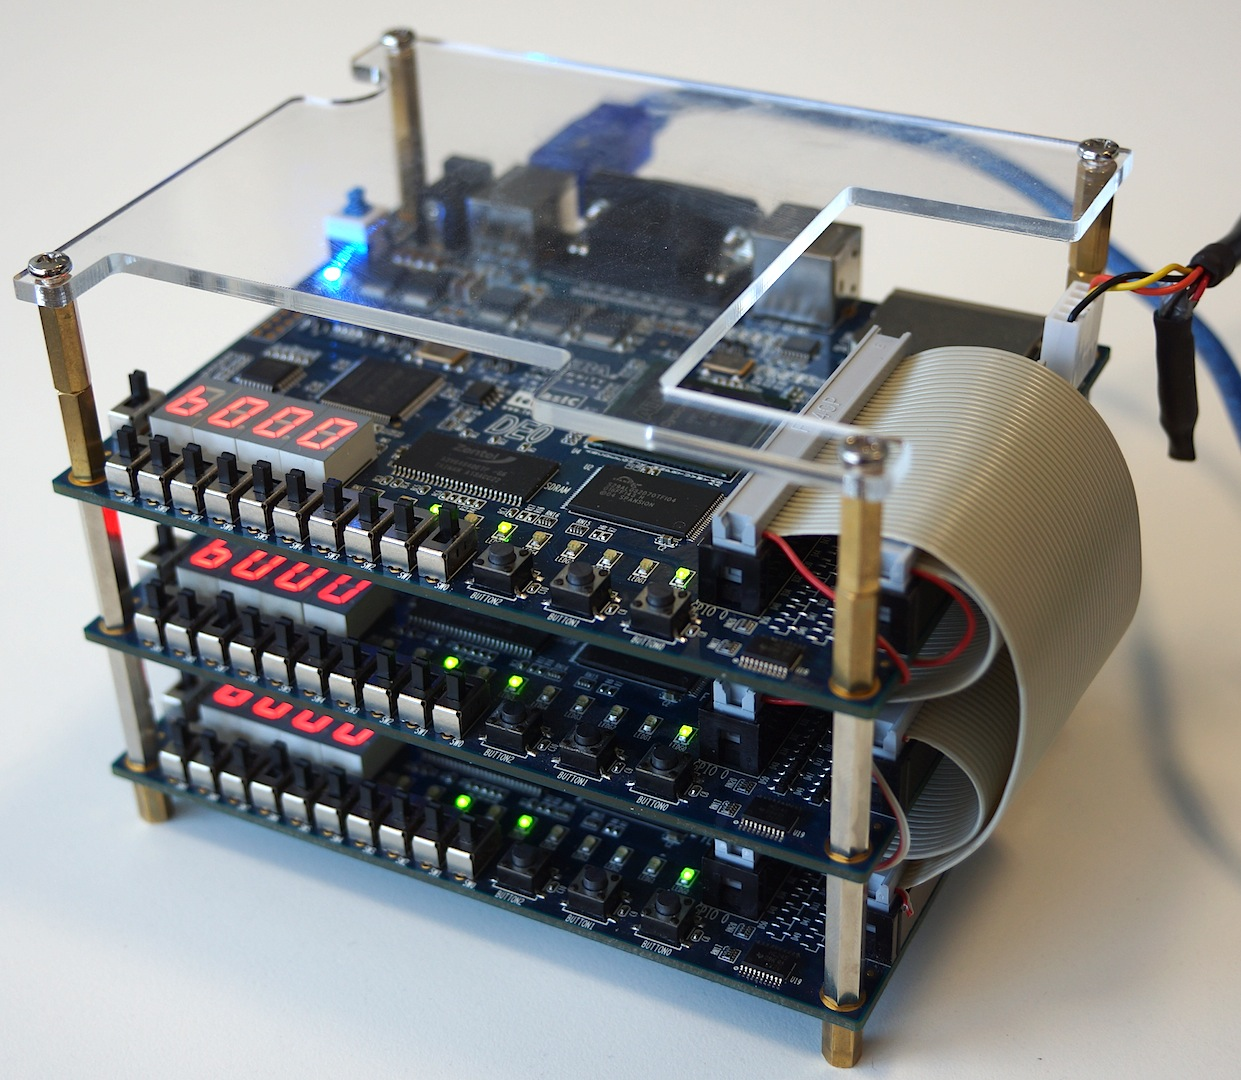
\includegraphics[width=\textwidth]{./figs/cluster.jpg}
  \caption{Hardware Implementation}
\end{figure}

\begin{figure}[p]
  \includegraphics[width=\textwidth]{./figs/interfpga.pdf}
  \caption{Inter-FPGA Communication Hardware Setup}
\end{figure}

\section{Programming the FPGA Devices}


The FPGA device images is the setup information that dictates how the FPGA functions. In order to do this, 2 images must be compiled. One image will go on the slave, one on the master. The master is the device that produces the clock and is connected to the UART as detailed earlier. This is done in the Altera Quartus II software with the two projects made available on request. 
\subsection{Customising the Algorithm}

Any customisations to read length, pixel count or genome length must be done with the devices images. These are all done in the Parameters.vhd file. In this file all settings can be customised, default settings are listed in appendix \ref{App:default}. Once these are modified the two images are compiled. 

If the hardware setup is non-standard the pin planner should be used to define which pins each port should be connected to. This is done on Assignments $>$ Pin Planner page using relevant data from the hardware datasheet generally available from the manufacturer. 


\subsection{Compiling the Images}

The majority of the compilation work is done by Quartus. The image is compiled by running the compilation, at which point an output SOF file is produced, this is an image that can be stored in the RAM of the FPGA device. This then needs to be converted to an image that can be stored permanently on the FPGA device (not cleared when power is lost). This is done using Quartus' converter by going to File $>$ Convert Programming Files... with settings stored in MASTER.cof and SLAVE.cof files. Once this is done, the Quartus programmer can be used to program the devices.


\subsection{Programming the Devices}

The devices are programmed in Programming mode entered by turning the power off, switching the programming switch shown in figure \ref{fig:de0} and turning power on with the USB BLASTER cable plugged in. Using the Quartus programmer (found in Tools $>$ Programmer) each device should be programmed with the POF image produced by the converter using the Active Serial mode. Once all devices have been programmed, each device should be returned to run mode using the switch and the reset should be pressed on the master device.

At this point the switches 6 to 9 should be set to the binary value indicating the order of the device in the cluster.

\textbf{\textit{NB. Once these tasks are complete the running of the comparison engine can be run as many times as wanted without reprogramming.}}

\section{Running The Comparison}

Having programmed the devices, it is now possible to run the comparison using the python script or program provided. This should be done from the command line, navigating to the location of the executable. The program should be run with the following arguments: Location of input file, number of pixels, read length. The input file should follow the format listed in Chapter 4 Section 3- Host Software. For example ``Testbench.exe dna.text 27 50''. This will trigger the comparison engine to run, returning the output data to a time stamped text file in the directory of the program. The output data will also be in the format listed in Chapter 4 Section 3. 